\documentclass[9pt,twocolumn,twoside]{styles/osajnl}
\usepackage{fancyvrb}
\journal{i524} 

\title{Cassandra}

\author[1]{Sabyasachi Roy Choudhury}

\affil[1]{School of Informatics and Computing, Bloomington, IN 47408, U.S.A.}

\affil[*]{Corresponding authors: sabyasachi087@gmail.com}

\dates{project-000, \today}

\ociscodes{Cloud, I524}

% replace this with your url in github/gitlab
\doi{\url{https://github.com/cloudmesh/sp17-i524/raw/master/paper2/S17-IO-3015/report.pdf}}


\begin{abstract}
Apache \href{http://cassandra.apache.org/}{Cassandra} is a `NoSql` database meant to 
handle a large volume of data through use of commodity hardwares. In this paper we examine
Cassandra by understanding the architecture and internal data flows.\newline
\end{abstract}

\setboolean{displaycopyright}{true}

\begin{document}

\maketitle

\section{Introduction}

Apache Cassandra is an open source column-oriented database that bases its distribution design on Amazon’s Dynamo and its data model on Google’s Bigtable {`cite:`cassandra-book}. It was developed by Facebook to handle large volume of writes and fault tolerance. The choice of database is solely on the basis of requirements. Cassandra is meant for scalability. If the need is to support thousands of write operations with millions of records, Cassandra or any other column oriented database  is much more suitable. But if your need is to support transactions and considerably lower read/write access, RDBMS (Relational Database Management System) is best suited.

\subsection{Column Oriented Database}

Column Oriented Database {`cite:`www-column-db} uses columns to store data tables rather than using rows as in traditional RDBMS. The main difference between column and row approach is schema definition. Column oriented databases have flexibility in column, in which it is not necessary for all the rows have same columns structure, but in RDBMS they are fixed and same for all the rows.

\section{Terminologies}

\begin{description}
  \item[Partitioning] \cite{www-dzone}Cassandra is a distributed system where data is distributed across multiple nodes. Each node is responsible for a part of the data.
  \item[Replication] \cite{www-dzone}In a distributed architecture, if one node is down , one of the data source is also sacrificed along with it. To avoid this, data in each node is copied to multiple nodes ensuring fault truculence and resulting in no single point of failure.
  \item[Gossip Protocol] \cite{wiki-gossip}Since Cassandra is a distributed system, it is important for individual nodes to know the existence and state of each other. To do so , Cassandra uses Gossip protocol.
  \item[Memtable] \cite{www-dzone}It is an In-Memory-Table or a write back cache in which data has not yet flushed into disk.
  \item[Column Family] \cite{wiki-columnfamily}It is a NoSql object to store key-value pair. Each column family has one key mapped with set of columns. Each column contains column name , its value and timestamp.
  \item[Bloom Filters] \cite{www-dzone}This algorithm helps to determine of a key is not present in a specific location. This helps in reducing I/O operations.
\end{description}

\section{Architecture}

\subsection{Cassandra Cluster/Ring}

We have already covered that Cassandra is a distributed system. Each node of the system is assigned with an id or name to uniquely identify it. The set of nodes which helps Cassandra to start up, are know as seeds. Cassandra uses this seed to retrieve informations about other existing nodes. It uses gossip protocol for intra node communication and failure detection. A node exchanges state informations only to other three nodes. This state information contains data about itself and about other known three members reducing IO operations.

\begin{figure}[h]
\begin{center}
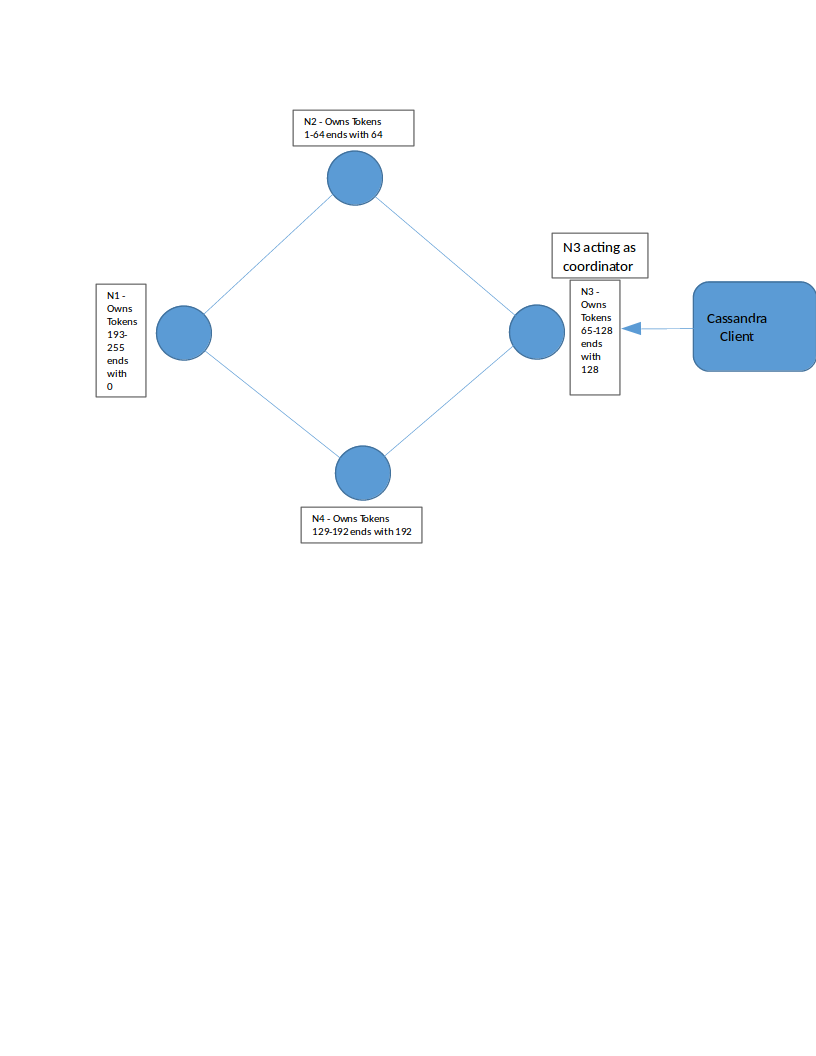
\includegraphics[width =3in,height=2.5in]{images/Cassandra_Ring_figure1}
\caption{Cassandra Cluster Ring}
\label{fig:figure1}
\end{center}
\end{figure}

\subsection{Data Distribution and Replication}

Each node of Cassandra, is responsible for a specific range or set of data. During the start-up, every node is assigned with range of token ensuring evenly distribution of data. In figure \ref{fig:figure1}, 0-255 range of data is distributed in four nodes. Hashing technique reviewed earlier is use to create the token of the row key. The row key falling under any of the above shown range will be assigned to its corresponding node. Say for example if the hash value of the row key comes to 38 , it will go to the node N2. 
In a distributed system, once can't rely on a single node for storing a set of data, as if the node is down that particular set won't be available for read, write and update. To achieve a better reliability and fault tolerance , Cassandra replicates data in multiple nodes. It has two basic replication strategy : 
\begin{enumerate}
     \item Simple - In this data is copied on to the next node in a clockwise manner
     \item Network-Topology - In this Cassandra is aware of the node's     
\end{enumerate}

\subsection{Read and Write Paths}

\begin{figure}[h]
\begin{center}
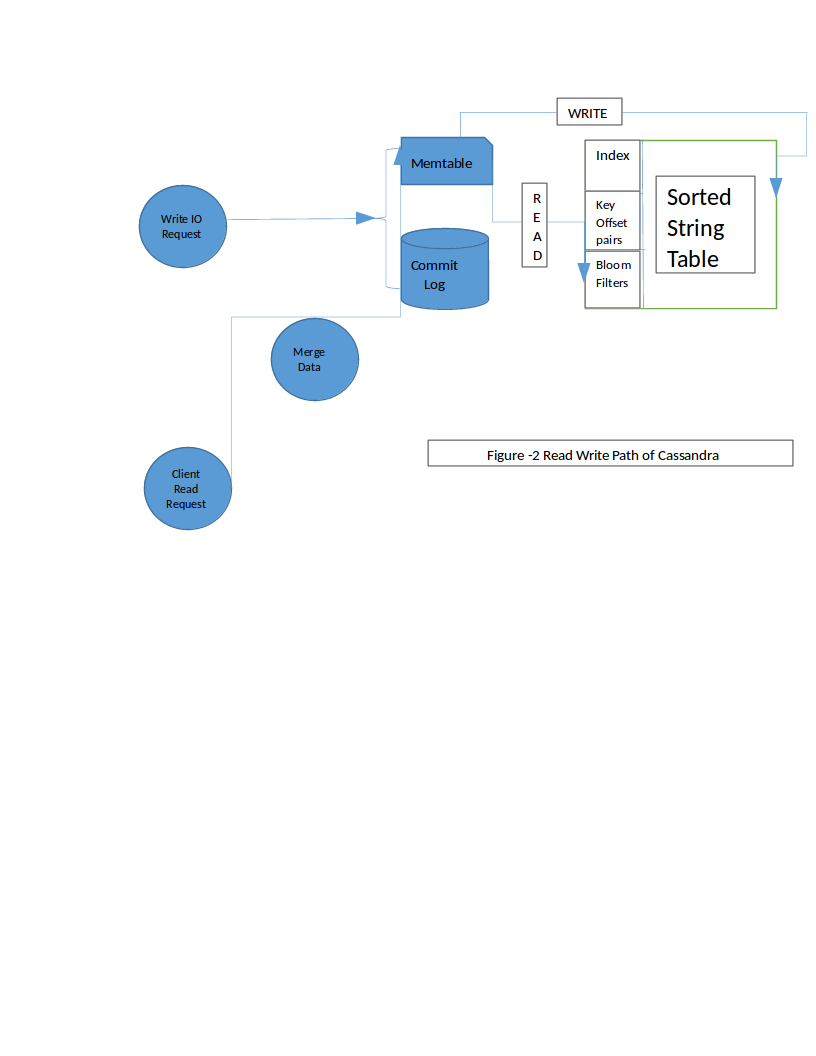
\includegraphics[width =3in,height=2.5in]{images/Cassandra_Write_Read_figure2}
\caption{Cassandra Read Write Data Flow}
\label{fig:figure2}
\end{center}
\end{figure}

In figure \ref{fig:figure1}, the client is connected with node 3. Since Cassandra is master less, N3 will be acting as coordinator and will serve for all client requests. It is the responsibility of N3 to communicate with its fellow nodes and fetch the desired results. We have already discussed that not all nodes communicates will all others for data retrieval instead it communicates only with handful of nodes for reducing IO operations. The number of nodes to communicate can be configured using QUORUM or knows as consistency level.
Read and write flows has been described in figure \ref{fig:figure2}. Each node processes write requests separately. It writes the data to Commit log first and then to Memtable. In case the node crashes, data can be restored from the Commit log. The data from Memtable will only be flushed to the disk or SSTable if 
\begin{enumerate}
     \item It reaches its maximum allocated size in memory
     \item The number of minutes a memtable can stay in memory elapses.   
     \item Manually flushed by a user  
\end{enumerate}
Read operation is similar to write operation. Every read operation must be with row key. As discussed earlier, row-key is used to determine the right node and the request is then passed to that particular node. Read is then catered by the bloom-filter and then proceeds to the desired result set.

\section*{Acknowledgments}

I would like to thanks Akhil Mehra for his vibrant description of Cassandra architecture.

% Bibliography

\bibliography{references}

\end{document}
